\documentclass[a4paper]{article}

\usepackage[top=2.5cm, bottom=3.5cm, left=2.5cm, right=2.5cm]{geometry}
\usepackage[utf8]{inputenc}
\usepackage[T1]{fontenc}
\usepackage[macedonian]{babel}
\usepackage[parfill]{parskip}
\usepackage{graphicx}
\usepackage{amssymb}
\usepackage{amsmath}
\usepackage{listings}
\usepackage{caption}
\renewcommand{\lstlistingname}{Код}

\usepackage{xcolor}
\usepackage{pgfplots}
\pgfplotsset{compat=1.18}

\usepackage{setspace}
\usepackage{lipsum}
\usepackage{fancyhdr}
\usepackage[hidelinks]{hyperref}
\usepackage{longtable}
\usepackage{array}
\usepackage{booktabs}
\usepackage{minted}
\setminted{
  style=friendly,
  fontsize=\normalsize,
  tabsize=2
}

\pagestyle{fancy}
\fancyhf{}
\fancyfoot[C]{\large \thepage}
\renewcommand{\headrulewidth}{0pt}
\setlength{\footskip}{15mm}

% Code listing style for Python
\lstdefinestyle{python}{
  language=Python,
  basicstyle=\ttfamily\small,
  keywordstyle=\bfseries\color{blue},
  commentstyle=\itshape\color{gray},
  stringstyle=\color{orange},
  numbers=left,
  numberstyle=\tiny\color{gray},
  stepnumber=1,
  frame=single,
  breaklines=true,
  showstringspaces=false,
  captionpos=b,
  xleftmargin=0.05\textwidth,
  xrightmargin=0.05\textwidth
}

\lstset{
  basicstyle=\ttfamily\small,
  keywordstyle=\bfseries\color{blue},
  commentstyle=\itshape\color{gray},
  stringstyle=\color{cyan},
  numbers=left,
  numberstyle=\tiny\color{gray},
  stepnumber=1,
  frame=single,
  breaklines=true,
  showstringspaces=false,
  captionpos=b,
  xleftmargin=0.05\textwidth,
  xrightmargin=0.05\textwidth
}



\newcommand{\UniversityName}
    {Универзитет „Св. Кирил и Методиј" во Скопје}
\newcommand{\FacultyName}
    {Факултет за информатички науки и компјутерско инженерство}
\newcommand{\ProjectType}
    {Дипломска работа}

\newcommand{\ProjectTitle}
    {Lyncis – IoT платформа за собирање и анализа на информации за работната околина}
\newcommand{\ProjectMentor}
    {Проф. д-р Игор Мишковски}
\newcommand{\ProjectCandidate}
    {Андреј Мицков}
\newcommand{\ProjectCandidateIndex}
    {216014}
\newcommand{\ProjectDate}
    {Декември 2025}


\begin{document}

    % Насловна страна
    \begin{titlepage}
    
    \begin{center}
        \setstretch{1.5}

        % Лого на УКИМ и ФИНКИ
        \begin{figure}[h]
            \centering
            \begin{minipage}{3cm}
                \centering
                
\includegraphics[width=3cm]{Miscellaneous/Logo-Ukim.png}
            \end{minipage}
            \begin{minipage}{3cm}
                \centering
                
\includegraphics[width=3cm]{Miscellaneous/Logo-Finki.jpg}
            \end{minipage}
        \end{figure}  

        % Име на универзитет и факултет
        \vspace{1em}
        {\Large \UniversityName} \\
        {\Large \FacultyName} \\

        % Тип на проект
        \vspace{2em}
        {\Large \textsc{\ProjectType}} \\

        \vfill

        % Наслов на проект
        {\Huge \textbf{\ProjectTitle}} \\

        \vfill

        \setstretch{1}
        % Ментор на проект
        \begin{minipage}[t]{.49\textwidth}
            \large \textbf{Ментор}\par 
            \ProjectMentor
        \end{minipage}
        \hfill
        % Автор на проект
        \begin{minipage}[t]{.45\textwidth}
            \large \hfill\textbf{Кандидат}\par 
            \hfill \ProjectCandidate \par
            \hfill \ProjectCandidateIndex
        \end{minipage}

        % Датум на изработка на проект
        \vspace{2cm}
        {\large \ProjectDate \vspace{-2mm}} 
        \rule{\textwidth}{0.5mm}
    \end{center}
    
\end{titlepage}


    \setlength{\parindent}{15pt}
    \fontsize{12pt}{14pt}\selectfont
    
    % Апстракт
    \newpage
\pagenumbering{roman}
\setcounter{page}{2}

\phantomsection
\addcontentsline{toc}{section}{Апстракт}

\begin{center}
    {\Large \textbf{Апстракт}}
\end{center}

\vspace{0.5cm}

Во овој дипломски труд обработувам практична и актуелна тема од
денешницата: следење и подобрување на здравата работна околина и
поддршка на здравјето на вработените во модерните работни простори.
Секојдневието на инженерите често вклучува долги часови работа во
затворени простории, при што малите промени во квалитетот на воздухот и
удобноста можат да предизвикаат замор, намалена концентрација и пад во
ефикасноста. Потребен е систем кој автоматски ги следи овие параметри и
овозможува навремена анализа, со што и навремена реакција за подобрување
на состојбата. Така во рамките на овој дипломски труд изработувам IoT
(Internet of Things) систем која прибира податоци од повеќе различни
извори: сензори за околината, Android паметни уреди како и надворешни
сервиси за временска прогноза и загадување. Системот обезбедува
автоматизирано следење, собирање, визуелизација како и обработка со
помош на вештачка интелигенција. Платформата е изработена врз
микро-сервисна архитектура, користејќи MQTT како главен протокол за
комуникација измеѓу уредите и платформата, взаемна автентикација со TLS,
\texttt{Redis Streams} за непречена проток на отчитувањата до \texttt{TimescaleDB} базата
на податоци, а врз сето тоа развиена е и веб контролна табла, сервис за
интелигентна анализа на собраните податоци со помош на вештачка
интелигенција, како и Android апликација што овозможува прибирање на
фитнес податоци. На овој начин, развиената платформа претставува
целокупен пристап за објективно мерење, анализа и интерпретација на
различните фактори кои влијаат врз продуктивноста и здравјето во
модерните работни простории.

\vspace{0.5cm}

\textbf{Клучни зборови:} \textit{IoT, MQTT, mTLS, микросервиси, TimescaleDB, вештачка интелигенција, работна околина, телеметрија.}


    % Содржина
    \newpage
    \renewcommand{\contentsname}{\LARGE Содржина}
    \tableofcontents

    % Вовед
    \newpage
\pagenumbering{arabic}
\setcounter{page}{1}

\section{Вовед}

Во современите работни простории се посветува сè поголемо внимание врз
квалитетот на работната околина и здравствените навики на работниците,
особено кај инженерите и ИТ професионалците кои се долго време во
затворени простории како и пред компјутер на своите бироа. Најразличните
параметри како температура, влажност на воздухот, светлина,
концентрација на различни гасови како CO2, NO2, CO, бучавата и
осветлувањето во просторијата имаат значајна улога во продуктивноста,
фокусот па и општата благосостојба на човекот, но во најголемиот дел од
компаниите тие не се следат континуирано или објективно. Токму оваа
потреба, мене лично, а и на другите околу мене за подобро и подетално
разбирање на условите во работната средина претставува основна
мотивација за развој на оваа платформа која овозможува автоматизирано
прибирање, визуелизација и анализа на релевантни податоци.

На пазарот постојат повеќе решенија за IoT мониторинг, но секое од нив
има свои ограничувања. Home Assistant е популарна open-source платформа
која овозможува интеграција на различни паметни уреди, но бара
комплексна конфигурација и техничко знаење за поставување, а не
обезбедува вградени механизми за безбедна автентикација на уредите.
Комерцијалните решенија како AWS IoT Core и Azure IoT Hub нудат напредни
enterprise функционалности, решенија и висока скалабилност, но нивната
цена и комплексност ги прават непрактични за индивидуална употреба или
мали организации. ThingsBoard претставува добра платформа за
визуелизација на IoT податоци, но нема вградена интеграција со модели за
вештачка интелигенција за напредна анализа. Од друга страна,
здравствените платформи како Google Fit, Samsung Health, Mi Fitness и
други, работат во затворени екосистеми и не дозволуваат едноставна
интеграција со околински сензори или сопствени системи.

Иако постојат многу поединечни решенија за мониторинг на одделни
параметри, или пак можност за интеграција на разни уреди, ниту еден од
нив не претставува интегриран систем кој истовремено ги спојува
околинските услови, здравствените навики на корисниците како и
надворешните услови како временска прогноза или квалитетот на воздухот.
Дополнително, се соочуваат со разни проблеми како недоволно интуитивен и
напреден кориснички интерфејс, небезбеден начин на испраќање на
информациите, како и неефикасен начин на складирање на собраните
податоци. Овие недостатоци создаваат простор и потреба за посеопфатно и
безбедно решение.

Целта на овој дипломски труд е да се изработи скалабилна, безбедна и
интуитивна платформа за автоматизирано прибирање, складирање,
визуелизација и анализа на податоци од сите достапни извори, со што се
добива увид со широк спектар за работната околина, условите во неа, како
и за самиот работник. Специфичните цели на проектот се:

\begin{itemize}
\item
  Дизајн и имплементација на микросервисна архитектура која овозможува
  модуларност и независно скалирање на компонентите
\item
  Имплементација на безбедна комуникација помеѓу уредите и платформата
  со взаемна TLS (mTLS) автентикација и X.509 сертификати
\item
  Развој на ефикасен систем за прием и складирање на временски податоци
  користејќи \texttt{Redis Streams} и \texttt{TimescaleDB}
\item
  Интеграција на сервис за анализа и интерпретација на собраните
  податоци со помош вештачка интелигенција и машинско учење
\item
  Изработка на интуитивна веб контролна табла со прилагодливи widgets за
  визуелизација и приказ на информациите
\item
  Развој на Android апликација за прибирање и испраќање на здравствени и
  фитнес податоци
\end{itemize}

Во втората глава од овој дипломски труд ја разгледувам теоретската
основа потребна за разбирање на системот: IoT концептите, MQTT
протоколот, безбедносните механизми со mTLS и X.509 сертификати,
микросервисната архитектура и временските бази на податоци. Во третата
глава го претставувам дизајнот на системот, вклучувајќи ја
архитектурата, протокот на податоци, безбедносниот модел и дизајнот на
базата на податоци. Четвртата глава е посветена на имплементацијата на
сите компоненти: сервисите за управување со уреди, прием на MQTT пораки,
запишување во база, вештачка интелигенција, веб контролната табла и
Android апликацијата. Во петтата глава ги прикажувам резултатите од
тестирањето и работата на системот, а во шестата глава го сумирам
заклучокот и предлагам идни насоки за развој.


    % Основи на IoT и применети технологии
    \newpage

\section{Основи на IoT и применети технологии}

Ова поглавје ги опфаќа основните технички концепти врз кои се базира
развиената платформа. Прикажани се клучните технологии, протоколи и
архитектонски принципи што овозможуваат безбедно, сигурно и скалабилно
функционирање на системот. Со разбирање на овие теоретски основи станува
појасно зошто одредени технолошки решенија се избрани и како тие
директно придонесуваат кон целокупната архитектура и функционирањето на
самата платформата.

\subsection{Интернет на Нештата}

Интернет на нештата (Internet of Things или IoT) претставува технолошки
концепт кој се однесува околу поврзување на голем број мали уреди со
интернетот со цел размена на податоци, обработка и автоматизација на
истите. Терминот прв пат е воведен кон крајот на 90-тите од страна на
Кевин Ештон, професор од МИТ. А во последните години достигнува голема
популарност со порастот на интернетот, зголемената достапност на
електронски компоненти, нивното поевтинување како и нивното усовршување
што овозможува полесна и поевтина имплементација на истите. Денес се
проценува дека во 2025 година постојат околу 20 милијарди IoT уреди, а
се проценува дека нивната бројка ќе се искачи до над 30 милијарди до
2030та година. IoT наоѓа широка примена во индустрија, здравство,
транспорт, земјоделие, паметни домови и многу други области.

Архитектурата на IoT системите најчесто се состои од три главни слоеви:
Perception, Network и Application слојот. Perception слојот ги опфаќа
сите уреди со сензори и актуатори кои се поставени во некоја околина,
Network слојот, односно мрежниот слој е слојот кој е задолжен за пренос
на информациите од и до самите уреди преку разни мрежни технологии како
WiFi, Bluetooth, 4G/5G, LoRaWAN како и други поедноставни радио
протоколи, како и специјализираните протоколи за истите како MQTT, HTTP,
AMQP. А додека пак Application слојот, односно апликацискиот претставува
највисокото ниво, и тој слој е задолжен за обработка, собирање,
складирање, анализа, прикажување на податоците од и за уредите.

Покрај широката примена, IoT системите и индустријата имаат бројни
предизвици. Еден од нив е безбедноста, бидејќи најчесто уредите се со
мала процесорска моќ и батериски напојувани не можат да извршуваат
комплексни криптографски операции. Скалабилноста претставува огромен
проблем бидејќи во IoT системите се очекува да комуницираат истовремено
стотици, а некогаш и илјадници. Интероперабилноста е исто клучен фактор
за успех, најчесто таа е ограничена од разни стандарди и протоколи кои
често знаат да се лиценцирани и приватни. Справувањето со големиот
волумен на податоци е исто така доста сложено, што бара специјализирани
системи за обработка и посебни бази на податоци за истите.

Сите овие предизвици се релевантни и за развиената платформа во овој
труд. Потребата за сигурна комуникација се адресира со имплементација на
mTLS и X.509 сертификати. Скалабилноста и ефикасното управување со
податоците се постигнуваат со користење на \texttt{Redis Streams} и \texttt{TimescaleDB},
додека микро-сервисната архитектура обезбедува флексибилност, независно
развивање и лесно проширување на системот. Со тоа, избраната архитектура
директно ги решава клучните слабости во традиционалните IoT решенија.

\subsection{MQTT}

Со ефикасност и сигурност како цел во преносот на телеметриските податоци
во IoT светот, изборот на комуникацискиот протокол има клучна улога. За
разлика од де факто стандардот за веб комуникација, HTTP, протокол кој
се базира на request/response моделот, MQTT (Message Queuing Telemetry
Transport) користи publish/subsrcibe модел, што го прави погоден за
системите со голем број на уреди и ограничени ресурси. MQTT е развиен
токму за овие намени, за средини со нестабилна мрежна конекција, мал
проток и уреди со ограничена процесорска и енергетска моќ, што го прави
идеален кандидат за IoT системи.

За разлика од HTTP, каде клиентот мора постојано да испраќа барања за да
провери дали има нови податоци, MQTT работи на принципот
publish/subscribe. Уредите кои се „произведуваат`` податоци(publishers)
ги испраќаат пораките до централен сервер наречен \texttt{broker}, додека
апликациите кои сакаат да ги „конзумираат`` тие податоци subscribers, се
претплатуваат на одредени теми. На овој начин, \texttt{broker}-от автоматски ги
доставува пораките до сите заинтересирани корисници без тие константно
да испраќаат барања.

Комуникацијата преку MQTT е организирана преку така наречени теми
(topics), кои имаат хиерархиска структура и овозможува организација на
пораките. На пример, тема од облик devices/sensor01/temperature јасно
укажува дека пораката се однесува на температура измерена од конкретен
уред. MQTT дополнително поддржува и т.н. wildcard знаци, со што се
овозможува флексибилно претплатување на повеќе теми истовремено, што е
особено корисно во системи со голем број уреди.

Исто така многу важен механизам кај MQTT е Quality of Service(QoS), кој
го дефинира нивото на сигурност при достава на пораките. Протоколот
поддржува три нивоа на QoS, кои овозможуваат баланс помеѓу брзината на
комуникација и сигурност во доставата. Овој механизам е особено битен
кај системи каде е важно пораките да не се изгубат, но истовремено да не
се оптоварува мрежата.

Покрај овие можности, MQTT нуди и дополнителни механизми како retained
пораки и last will пораки. Retained пораките се пораки кои остануваат во
\texttt{topic}-от, и секој нов претплатник ќе ја добие таа порака, за разликата
од другите нормални пораки кои ги добиваат само ако биле претплатени во
истиот момент кога била испратена. Додека пак last will пораката
претставува начин еден испраќач (publisher) кога непланирано ќе се
дисконектира да остави некаква трага. Благодарение на овие
карактеристики, MQTT претставува стандарден избор за комуникација во IoT
платформите, вклучувајќи го и платформата која ја развивам во рамките на
овој дипломски труд.

\subsection{Безбедност - mTLS и X.509 сертификати}

Безбедноста претставува еден од најкритичните аспекти кај IoT системите,
бидејќи уредите најчесто се поставени на небезбедни локации и
комуницираат преку небезбедни канали. Во изминатите години се забележани
бројни напади врз IoT уредите, каде илјадници уреди се компромитирани
поради слаба софтверска безбедност. Денес тие претставуваат една од
главните мети на хакерски напади поради нивното сѐ присуство и
ранливост. Еден таков познат напад е Mirai botnet во 2016, преку кој беа
компромитирани стотици илјади уреди поради користење слаби лозинки или
стандардни лозинки. Поради таквите примери класичната добро позната
автентикација со лозинка и корисничко име се смета за не соодветно
решение.

За заштита на комуникацијата кај IoT уредите се користи TLS (Transport
Layer Security) протоколот, кој обезбедува енкрипција на податоците,
интегритет и автентикација на двете страни во комуникацијата. При TCP
конекција, TLS спроведува размена на сертификати за потврда на
идентитетот. Kај стандардниот TLS, како на пример за web комуникација,
се врши еднострана идентификација, односно серверот се идентификува пред
клиентот за да покаже дека тој е стварно тој, додека пак кај mutual TLS
(mTLS) и клиентот и серверот меѓусебно се автентицираат. Ова е посебно
важно кај IoT уредите, бидејќи секој уред мора да биде јасно
идентификуван со што се спречува неовластен пристап до системот.

Автентикацијата кај mTLS се заснова врз X.509 дигитални сертификати.
Секој сертификат содржи податоци за сопственикот, јавен криптографски
клуч, неговата важност, неговиот сериски број како и дигитален потпис од
доверлив издавач, односно така наречен Certificate Authority (CA). Преку
концептот наречен „ chain of trust`` се обезбедува сигурност дека
сертификатот е издаден од валидна и доверлива институција,.

Во рамките на системот развиен за овој дипломски труд се користи интерен
Certificate Authority, преку кој се издаваат X.509 сертификати за секој
уред. Процесот на генерирање и управување со сертификати е имплементиран
во рамките на сервисот за управување со уреди (\texttt{device\_manager}), додека
пак MQTT \texttt{broker}-от врши верификација на сертификатите при секое
поврзување. Дополнително, се користи и Certificate Revocation List
(CRL), со што се овозможува одземање на пристапот на компромитирани или
неактивни уреди, што спречува користење на тие валидни цели за
малициозни цели.

Со примената на mTLS се обезбедува високо ниво на безбедност, доверлива
идентификација на уредите и заштита на податоците при нивниот пренос.

\subsection{Микросервисна архитектура}

Традиционалниот пристап во развојот на софтверските системи најчесто се
базира на монолитна архитектура, каде целата функционалност на една
апликација е имплементирана во една целина. Овој начин е доста
едноставен за почетна имплементација, но како што се зголемува
комплексноста и бројот на корисници, одржувањето, скалабилноста на
системот и развојот стануваат се потешки за менаџирање. Спротивно на тоа
микросервисната архитектура го дели системот на повеќе мали, логички
независни целини наречени сервиси, од кои секој извршува една точно
јасно дефинирана функција и комуницира со останатите најчесто преку
мрежа.

Главните предности на микросервисната архитектура се флексибилноста,
скалабилноста и можноста секој да се развива независно. Секој
микросервис може да се развива во различна насока, со различни
технологии и програмски јазици во зависност од потребата и намената.
Дополнително, проблем со еден од сервисите не значи дека и целиот систем
ќе престане со работа. Тоа дополнително ја зголемува отпорноста на
грешки на системот. Овој пристап е доста користен и погоден за IoT
системи, бидејќи различни компоненти имаат различни намени, барања за
перформанси и скалабилност.

Покрај своите бројни предности, микросервисната архитектура како и се
друго има и свои недостатоци и предизвици. Комуникацијата помеѓу
микросервисите се одвива преку мрежа, што може да доведе до дополнително
каснење и грешки. Дистрибуираните системи се потешки за управување и
синхронизирање во споредба со монолитната архитектура. Нивното
дебагирање и откривање на проблеми е доста покомплексно, бидејќи треба
следење и анализирање на повеќе сервиси кои работат одвоено.

За надминување на ваквите предизвици, во микросервисините системи често
се применува асинхрона комуникација преку message queue механизми. Во
рамките на оваа дипломска се користи \texttt{Redis Streams} како комуникациски
посредник помеѓу некои сервиси. Преку концептот на \texttt{consumer groups},
повеќе worker процеси можат паралелно да читаат и обработуваат еден ист
stream. Дополнително, обезбедува at-least-once достава, со што се
намалува ризикот од губење на податоци.

Во платформа која се развива како дел од оваа дипломска работа се
имплементирани повеќе микросервиси со јасно дефинирани одговорности.
Сервисот \texttt{device\_manager} е задолжен за регистрација на уредите и
управување со X.509 сертификати. \texttt{mqtt\_ingestion} сервисот го прима
телеметрискиот сообраќај и го запишува во \texttt{Redis Streams}. \texttt{db\_write}
сервисот ја презема улогата на обработка и запишување на податоците во
базата на податоци. \texttt{gpt\_service} е задолжен за паметна анализа на
собраните податоци со помош на вештачка интелигенција , додека Django ни
служи како позадина за веб-контролната табла и оркестрира и комуницира
со другите сервиси и базата на податоци во која се запишуваат
телеметриските податоци. Со ваквата организација, секој сервис има јасна
улога, што го прави системот модуларен, проширлив и лесен за одржување.

\subsection{Временски бази на податоци}

IoT системите генерираат голем број на податоци во кратки временски
интервали, што резултира со голем број на INSERT операции во базата на
податоци. Ваквиот тип на податоци најчесто се анализираат според
временски опсези, како последен час, последен ден или месец, а не според
нивните класични релациски односи. А исто така често се извршуваат
агрегациски функции, максимално и минимални вредности во временски
период. Поради ваквите карактеристики, најчесто користените релациски
бази на податоци не се оптимални за ваков тип на податоци без надградби
за оптимизација.

Како решение за управување со податоци од временски серии, во рамките на
дипломскиот труд се користи \texttt{TimescaleDB}, кој претставува екстензија за
\texttt{PostgreSQL} широко користената релациона база на податоци. Ова овозможува
користење на секојдневна релациона база заедно со временски серии на
податоци. Клучниот концепт кај оваа база се така наречените \texttt{hypertables},
кои овозможуваат автоматско партиционирање на податоците кои се
временски серии, според временската димензија и дополнителни клучеви, со
што се постигнува висока ефикасност за запишување и читање.
Дополнително, \texttt{TimescaleDB} поддржува компресија на стари податоци, што
помага за намалување на просторот кој го зафаќа базата на податоци, како
и континуирани агрегации (continous aggregations), кои овозможуваат
автоматско пресметување на агрегатни вредности по претходно зададени
временски интервали.

Во платформата развиена за овој дипломски труд, телеметриските податоци
се складирани во посебна \texttt{telemetry} табела, чија структура е прилагодена
на временската природа на податоците, односно е \texttt{hypertable}. Примарниот
клуч е составен од времето на мерење, идентификаторот на уредот и типот
на метриката, односно (time, device\_id, metric). Ваквиот редослед на
клучевите овозможува ефикасни пребарување најчесто користени во
системот, како на пример прикажување на податоци за конкретен уред во
одреден временски период.

Со прикажаните концепти за IoT, комуникациски протоколи, безбедност, микросервисна архитектура и временски бази на податоци се поставува теоретската основа за дизајнот на конкретниот систем. Во следното поглавје детално е опишана архитектурата на развиената платформа и меѓусебната интеракција на нејзините компоненти.

    % Дизајн на системот
    \newpage

\section{Дизајн на системот}

\subsection{Архитектура на платформата}

Развиената платформа е изградена врз микросервисна архитектура, со цел
да обезбеди висока скалабилност, добра флексибилност и отпорност на
грешки и проблеми. Наместо целата логика да е сместена во една монолитна
апликација, функционалноста е поделена во повеќе независни микросервиси
кои меѓусебно комуницираат преку мрежа. Ваквиот пристап овозможува
изолирање на одговорностите по сервиси, подобра контрола на ресурсите и
поедноставно одржување, додавање нови функционалности и скалирање.

Архитектурата на платформата е составена од повеќе специјализирани
микросервиси, од кои секој има јасно дефинира улога во целокупниот
процес. Сервисот \texttt{device\_manager}, имплементиран со \texttt{FastAPI}, е задолжен
за регистрација на уредите и управување со нивните X.509 сертификати.
Сервисот \texttt{mqtt\_ingestion} е одговорен за прием на MQTT пораките од
уредите и нивно проследување кон \texttt{Redis Streams}. \texttt{db\_write} сервисот ја
презема обработката на податоците од message queue и нивно запишување во
базата на податоци. \texttt{gpt\_service} овозможува интелигентна анализа на
собраните податоци со примена на вештачка интелигенција. Django служи
како комуникациски слој помеѓу сите микросервиси и frontend апликацијата
изградена со React која ни овозможува визуелизација на податоците,
интеракција со истите, и целосна табла за контрола со уредите.

При дизајнот на платформата беа во главно применети принципите на loose
coupling и single responsibility, со цел да се обезбеди јасна поделба на
одговорностите и минимална зависност меѓу сервисите. Секој микросервис
извршува една конкретна функционалност и комуницира со останатите
исклучиво преку дефинирани API-интерфејси или message queue механизми.
На овој начин се овозможува поедноставно тестирање, полесна интеграција
на нови функционалности и локализирано решавање на дефекти без да се
наруши стабилноста на целиот систем. Дополнително ваквиот пристап
овозможува независно хоризонтално скалирање на поединечни сервиси, во
зависност од реалното оптоварување, што е особено значајно за IoT
платформи со променлив број на активни уреди.

За размена на податоци помеѓу микросервисите задолжени за прием и
обработка на телеметриските информации е имплементиран асинхрон
комуникациски модел базиран на \texttt{Redis Streams}. Сервисот \texttt{mqtt\_ingestion}
функционира како producer и ги запишува сите пристигнати MQTT пораки во
централен stream, додека сервисот \texttt{db\_write} функционира како consumer и
ги чита пораките преку механизмот на \texttt{consumer groups}.

Ваквиот пристап овозможува откачување(decoupling) на сервисите на прием
и обработка, автоматско балансирање на товарот при повеќе активни worker
инстанции, како и задржување на пораките во случајот на привремен преки
или преоптоварување на downstream сервисите. Дополнително, \texttt{Redis Streams}
обезбедува at-least-once семантика, со што се намалува ризикот на губење
на телеметриските податоци. Целокупната комуникациска архитектура и движењето на податоците е прикажано на архитектурниот дијаграм (слика~\ref{fig:system-architecture}).

\begin{figure}[htbp]
    \centering
    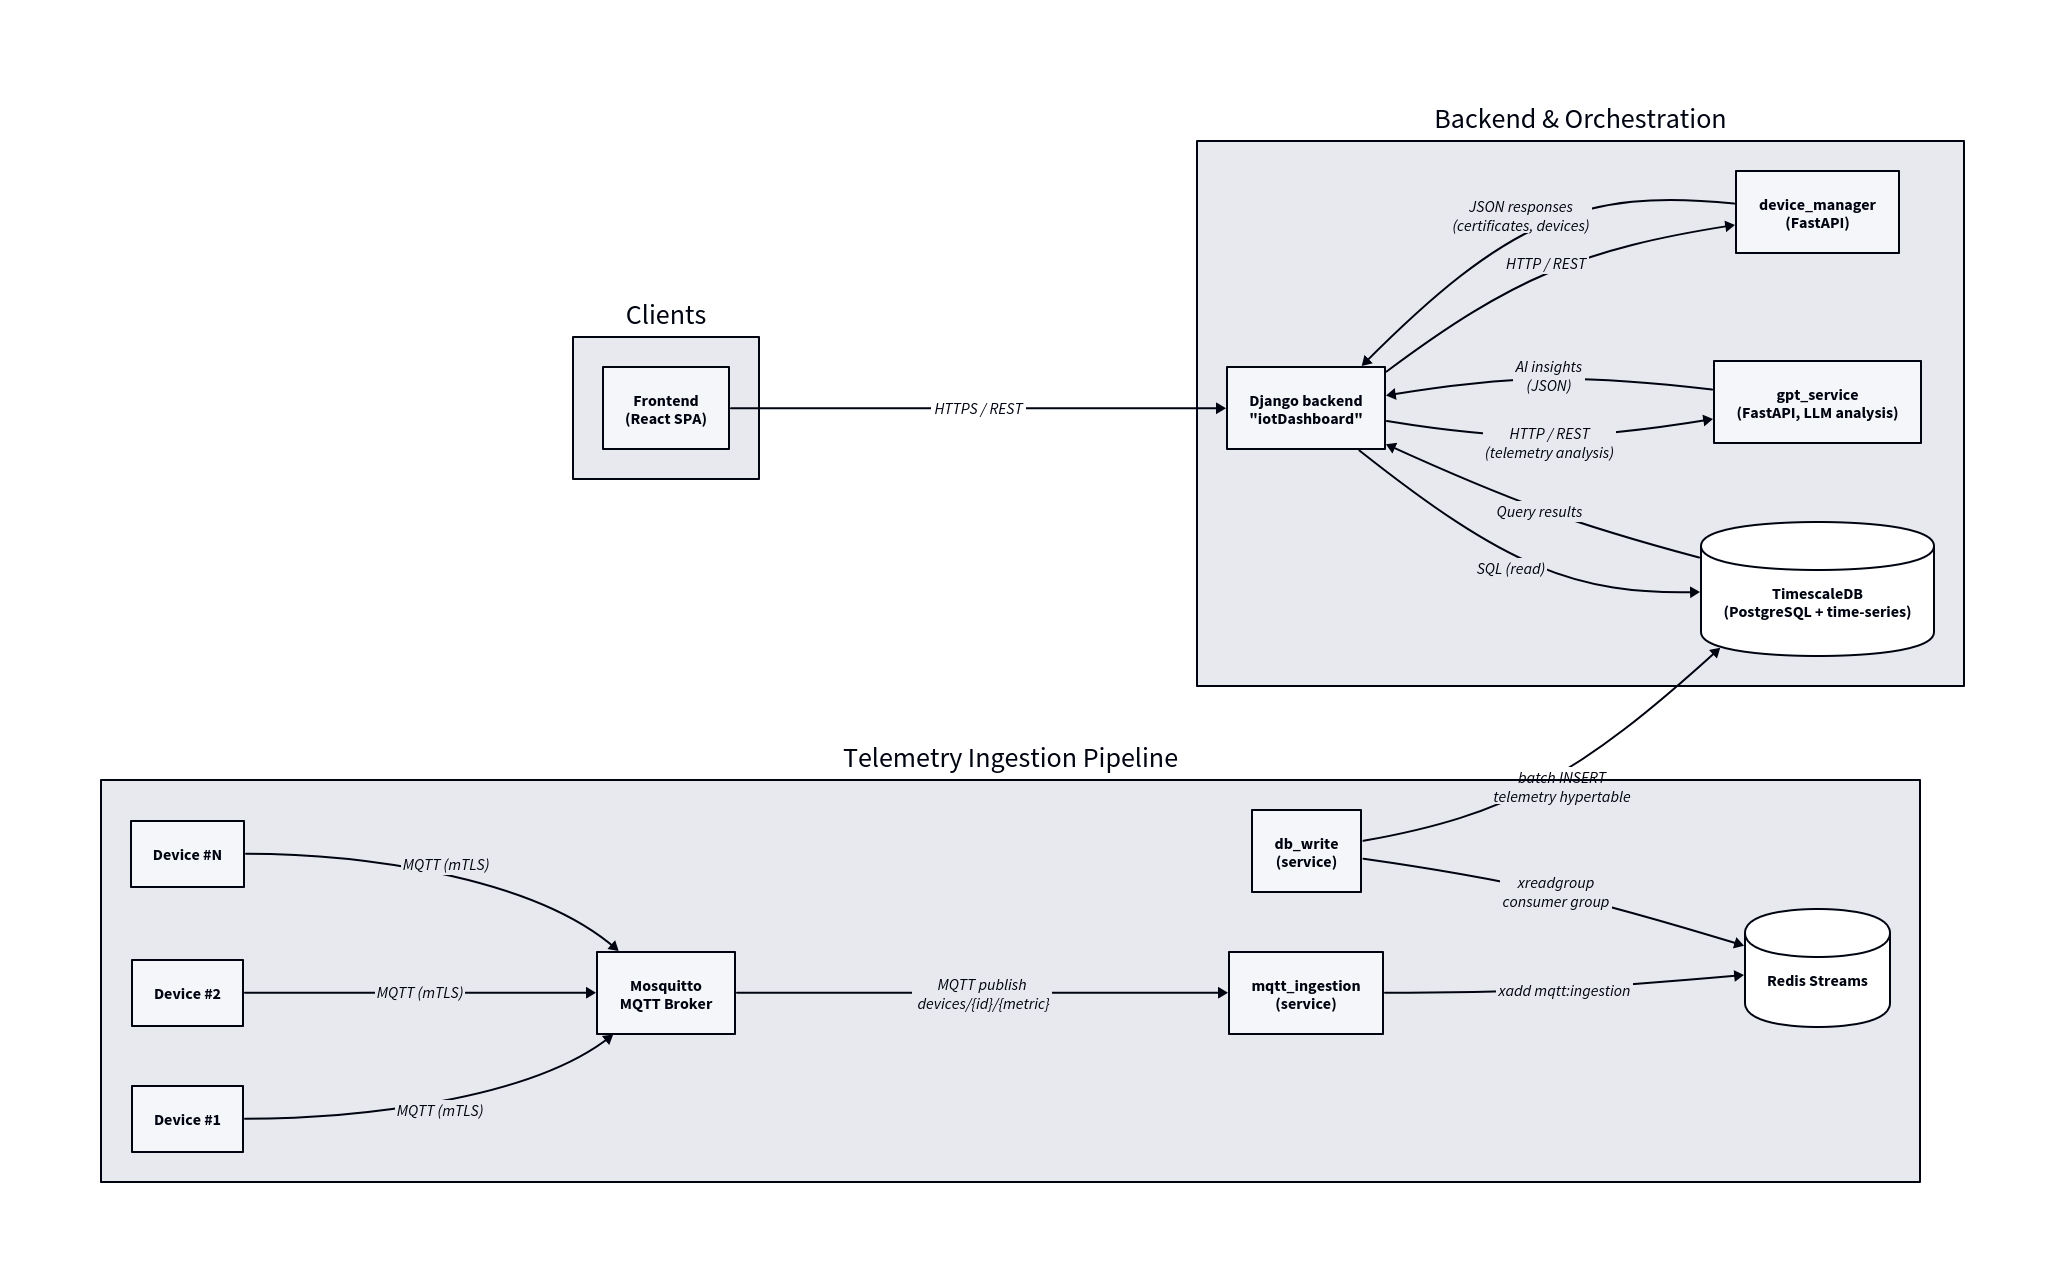
\includegraphics[width=\textwidth]{Miscellaneous/architecture.png}
    \caption{Архитектура на платформата за мониторинг на работна околина}
    \label{fig:system-architecture}
\end{figure}

\subsection{Проток на податоци}

Протокот на податоци во рамките на развиената платформа е дизајниран
така што овозможува сигурно, скалабилно и ефикасно движење на
информациите од крајните IoT уреди до веб интерфејсот. Процесот опфаќа
повеќе фази: регистрација на уред, безбедно поврзување преку mTLS,
испраќање и обработка на телеметриски податоци, нивно складирање во база
на податоци и конечно визуелизација преку frontend апликацијата.
Целокупниот тек е прикажан со дијаграм. (сл 3.2)

\subsubsection{Регистрација на уред}

Процесот започнува со регистрација на нов IoT уред во системот.
Корисникот иницира регистрација преку веб контролната табла имплементира
со React. При оваа постапка, frontend-от испраќа HTTP POST барање до
Django REST API кое содржи основни информации за уредот, како што се
име, локација и тип на уред.

Django го проследува ова барање кон интерниот \texttt{device\_manager}
микросервис, кој е задолжен за управување со уредите и нивните дигитални
сертификати. Device\_manager креира нов запис во табелата devices во
базата на податоци и иницира процес на генерирање на X.509 сертификат за
конкретниот уред. По успешното генерирање и потпишување на сертификатот
од страна на интерниот Certificate Authority (CA), приватниот клуч и
сертификатот му се враќаат на корисникот. Овие податоци понатаму се
имплементираат на самиот уред, со што тој станува подготвен за безбедно
поврзување на системот.

\subsubsection{Поврзување на уред преку mTLS}

По успешната регистрација, уредот иницира TCP конекција кон MQTT
\texttt{broker}-от преку порт-от 8883 кој е наменет за MQTT со SSL. При
воспоставување на конекцијата се извршува mTLS handshake постапка, при
што уредот го презентира својот X.509 сертификат пред \texttt{broker}-от, а
\texttt{broker}-от го презентира својот сертификат пред уредот.

\texttt{Mosquitto broker}-от врши верификација на сертификатот преку:

\begin{itemize}
\item
  Проверка на потписот од интерниот CA
\item
  Проверка на валидноста (датум на важност)
\item
  Проверка во Certificate Revocation List (CRL)
\end{itemize}

Доколку сите проверки се успешни, конекцијата се прифаќа и уредот добива
дозвола за publish. Во спротивно, доколку сертификатот е невалиден,
конекцијата автоматски се одбива.

\subsubsection{Испраќање и процесирање на телеметрија}

Откако уредот е успешно поврзан со MQTT \texttt{broker}-от, тој започнува со
публикување на телеметриски податоци на MQTT теми во облик
„devices/\{device\_id\}/\{metric\}`` каде што device\_id претставува
уникатен идентификатор на уредот, а metric го означува тимот на
измерениот параметар (на пр. Температура, влажност, CO2).

Сервисот \texttt{mqtt\_ingestion} е претплатен на сите релевантни теми и
функционира како централен приемник на сите MQTT пораки. По приемот на
секоја порака, податоците се парсираат и се запишуваат како нов запис во
Redis Stream-от \texttt{mqtt:ingestion}.

Сервисот \texttt{db\_write} функционира како consumer во рамките на \texttt{Redis}
\texttt{consumer group} и ги чита пораките од stream-от асинхроно. Податоците се
групираат и се запишуваат во \texttt{TimescaleDB} базата како нови записи во
\texttt{telemetry} \texttt{hypertable}. На овој начин се обезбедува висок проток на
податоци, buffering при оптоварување и at-least-once гаранција за
достава.

\subsubsection{Визуелизација и пристап до податоците}

Откако податоците се складирани во базата, тие стануваат достапни за
визуелизација преку веб-контролната табла. Frontend апликација направена
со React комуницира со Django REST API преку HTTP барања, при што API
слојот врши SQL барања за извлекување на податоците во зададените
временски интервали.

Добиените податоци се прикажуваат преку интерактивни графици, виџети и
табели, овозможувајќи им на корисниците да добијат увид во реално време
и историски во состојбата на работната околина и активностите.

\subsubsection{Интеграција на интелигентна анализа}

Покрај стандардната визуелизација, платформата овозможува интелигентна
анализа на податоците преку gpt\_service микросервисот. Овој сервис се
повикува директно со потребите податоци кои треба да ги обработи со
помош на AI модел и генерира текстуални анализи, препораки и детекција
на аномалии. Резултатите од AI анализата се прикажуваат во frontend
апликацијата како виџети што овозможува дополнителен слој на
интерпретација на постоечките податоци.

\subsection{Безбедносен модел на платформата}

Безбедноста е еден од клучните аспекти при дизајнот на оваа IoT
платформа, поради фактот што најголемиот дел од уредите се поставени во
небезбедни средини и комуницираат преку јавни мрежи. Класичната
автентикација, како што е споменато претходно, со корисничко име и
лозинка не е соодветна за вакви системи, бидејќи често претставува чест
извор на безбедности пропусти. Поради тоа, во рамките на оваа платформа
е имплементиран безбедносен модел базиран на mutual TLS (mTLS).

Кај mTLS, и клиентот (IoT уредот) и серверот (MQTT \texttt{broker}-от) меѓусебно
се автентицираат преку X.509 дигитални сертификати. На овој начин се
обезбедува двострана проверка на идентитетот, како и енкрипција и
интегритет на податоците при нивниот пренос. Секој уред поседува
уникатен сертификат, со што се овозможува прецизна идентификација и
контрола на пристапот до системот.

Во основата на овој модел се наоѓа интерен Certificate Authority (CA),
која ги потпишува сите сертификати во системот. Процесот на издавање на
сертификат се реализира преку \texttt{device\_manager} сервисот, кој при
регистрација на уред генерира сертификат и приватен клуч, ги складира
релевантните податоци во базата и му ги враќа на корисникот за
инсталација на уредот.

За управување со компромитирани или неактивни уреди се користи механизам
за повлекување на сертификати преку Certificate Revocation List (CRL).
При повлекување на сертификатот, тој се означува како невалиден во
системот, CRL листата се ажурира и MQTT \texttt{broker}-от автоматски го одбива
секој понатамошен обид за поврзување со тој сертификат.

Изборот на mTLS обезбедува високо ниво на безбедност, елиминација на
лозинки, силна криптографска идентификација на уредите и заштита од
напади како man-in-the-middle, што го прави овој пристап особено погоден
за IoT платформи.

\subsection{Дизајн на базата на податоци}

Складирањето на податоците во системот е дизајнирано така што овозможува
сигурно управување со уредите, дигиталните сертификати и телеметриските
мерења. Поради временската природа и големиот волумен на податоци,
базата на податоци е реализирана со \texttt{PostgreSQL} со \texttt{TimescaleDB}
екстензија.

\subsubsection{Табела \texttt{devices}}

Табелата \texttt{devices} ги содржи основните информации за секој регистриран
уред во системот во неа се складираат податоци како:

\begin{itemize}
\item
  Id - единствен идентификатор на уредот
\item
  name - име на уредот
\item
  Location - локација уредот
\item
  Created\_at - време на регистрација
\end{itemize}

Оваа табела претставува централна точка за поврзување на сите останати
податоци во системот

\subsubsection{Табела \texttt{device\_certificates}}

Табелата \texttt{device\_certificates} се користи за управување со X.509
сертификатите поврзани со уредите. Таа содржи:

\begin{itemize}
\item
  Id - сериски број на сертификатот
\item
  Device\_id - надворешен клуч кон табелата devices
\item
  Issued\_at - датум на издавање
\item
  Expires\_at -- датум на истекување
\item
  Revoked\_at - датум на повлекување (доколку постои)
\end{itemize}

Преку оваа табела се обезбедува информации за целиот животен циклус на
секој сертификат

\subsubsection{Табела \texttt{telemetry}}

Табелата \texttt{telemetry} претставува \texttt{TimescaleDB hypertable} и е
оптимизирана за складирање на временски серии од телеметриски податоци.
Таа содржи:

\begin{itemize}
\item
  Device\_id - идентификатор на уредот
\item
  Metric - тип на измерениот параметар
\item
  Value - измерена вредност
\item
  Timestamp - време на мерење
\end{itemize}

Податоците се автоматски партиционирани по време, што овозможува високо
ниво на ефикасност при внесување и пребарување на податоци. Примарниот
клуч е составен од (timestamp, device\_id, metric), што овозможува
оптимизирани прашалници при анализа на податоци по уред и временски
опсег.

\texttt{TimescaleDB} e избрана поради неколку технички предности како што се:

\begin{itemize}
\item
  Оптимизирана за работа со временски серии
\item
  Автоматска компресија
\item
  Континуирани агрегации за пресметка на просечни вредности
\item
  Скалабилност и компатибилност со \texttt{PostgreSQL}
\end{itemize}

Со ова се овозможува ефикасно, стабилно и долгорочно чување и користење
на телеметриските податоци од платформата. Целокупната структура на базата
на податоци е прикажана на ER дијаграмот (слика~\ref{fig:er-diagram}).

\begin{figure}[htbp]
    \centering
    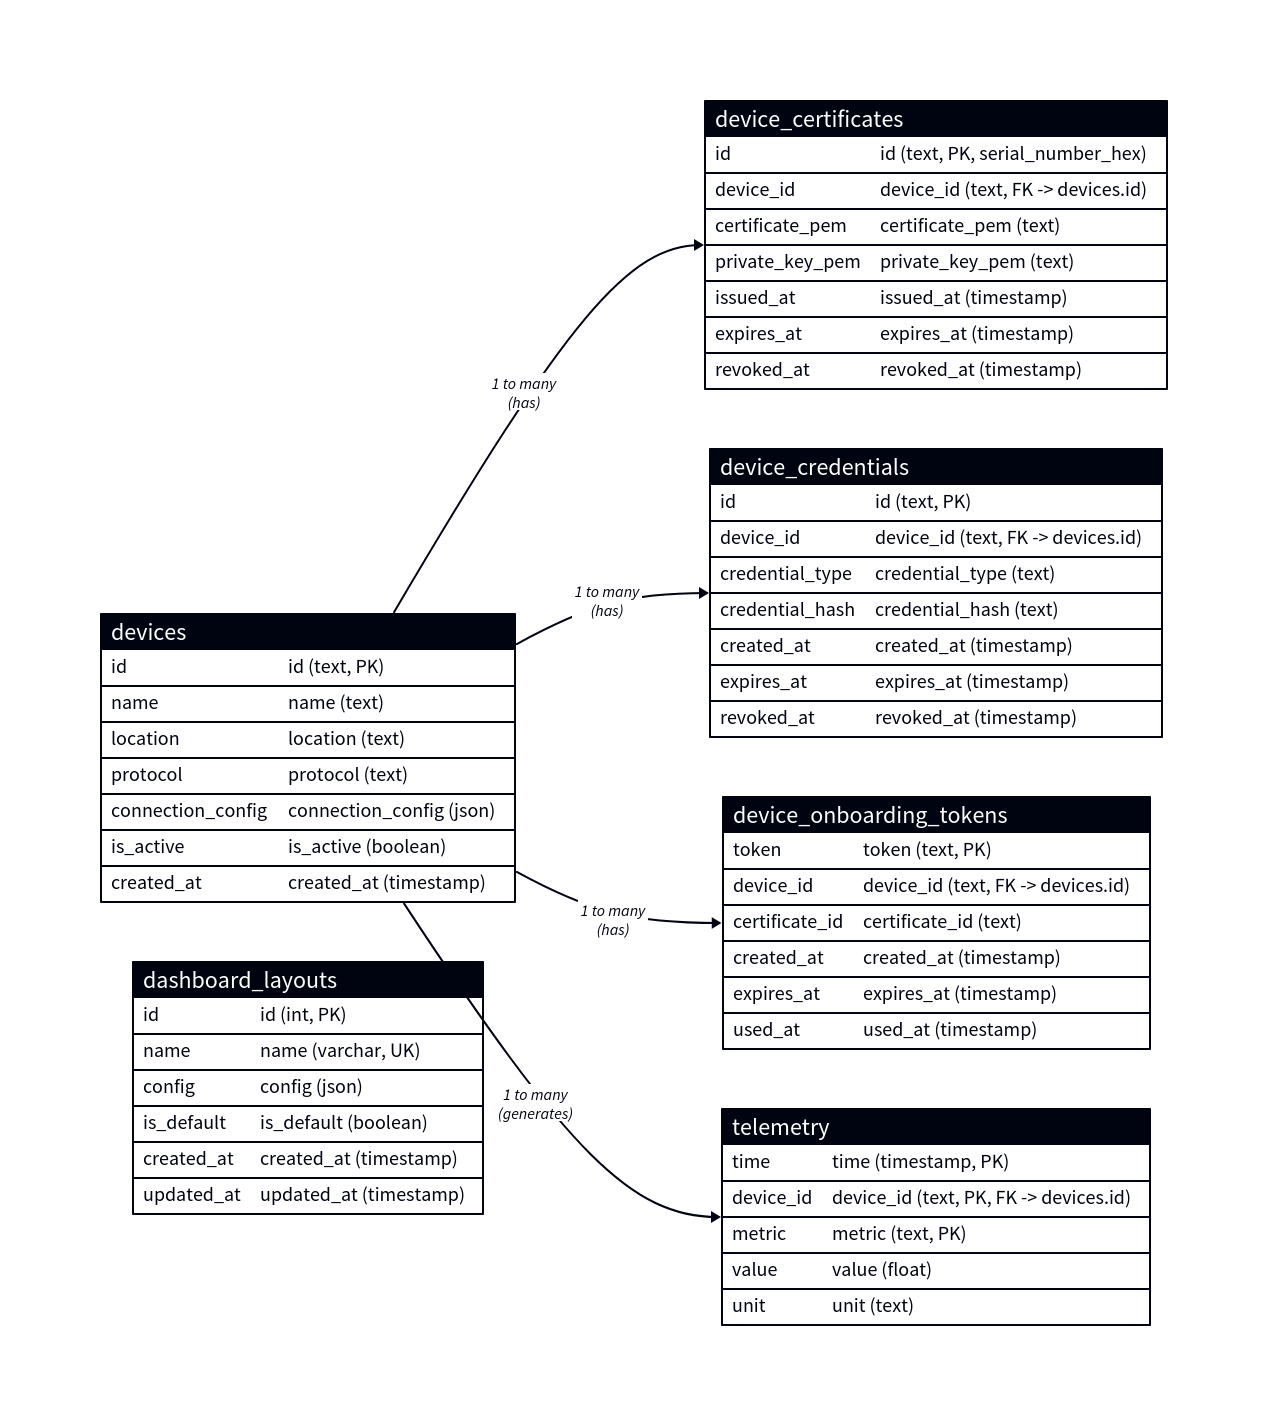
\includegraphics[width=\textwidth]{Miscellaneous/er_diagram.png}
    \caption{ER дијаграм на базата на податоци на платформата}
    \label{fig:er-diagram}
\end{figure}


    % Имплементација
    \newpage

\section{Имплементација}

Во оваа глава се прикажува практичната имплементација на платформата и
нејзината архитектура претходно опишана. Претставени се клучни делови од
backend-от, микросервисната инфраструктура и frontend апликацијата.
Ставен е акцент на најрелевантните и најинтересните сегменти кои
демонстрираат реализација на архитектонските одлуки, безбедносните
механизми и протокот на податоци низ системот.

\subsection{Backend имплементација}

Backend делот е имплементиран со користење на Django и Django REST
Framework (DRF) и претставува централна контролна точка за комуникација
помеѓу frontend апликацијата, микросервисите и базата на податоци.
Django REST API-то функционира како API gateway, преку кој се
реализираат сите операции поврзани со уредите, сертификатите,
телеметриските податоци и интелигентната анализа.

Иако системот користи \texttt{PostgreSQL} со \texttt{TimescaleDB} за складирање на
телеметрија, Django не управува со овие табели во write режим, Django
има read-only пристап, со што се избегнува мешање на Django ORM во
ingestion процесот, кој целосно се реализира преку микросервисите
mqtt\_ingestion и db\_write. Овој пристап овозможува висока
конзистентност, безбедно пишување на податоците и одвојување на
ingestion логиката од API слојот.

\subsubsection{Django REST API како комуникациски слој}

Django REST Framework (DRF) е искористен како централен комуникациски
слој помеѓу frontend апликација, микросервисите и базата на податоци.
Django API има улога на API gateway, преку кој се реализираат сите
надворешни барања од корисничкиот интерфејс, додека вистинската бизнис
логика (сертификати, AI анализа, ingest) е делегирана на посебни
микросервиси.

Во рамките на овој слој, за управување со уредите и телеметриските
податоци се користат DRF ModelViewSet и ReadOnlyModelViewSet. Основната
дефиниција е реализирана преку:

\begin{minted}{python}
class DeviceViewSet(viewsets.ModelViewSet):
    queryset = Device.objects.all()
    serializer_class = DeviceSerializer


class TelemetryViewSet(viewsets.ReadOnlyModelViewSet):
    """ViewSet for telemetry data queries."""
    
    queryset = Telemetry.objects.all()
    serializer_class = TelemetrySerializer
\end{minted}

DRF автоматски обезбедува CRUD операции, додека другите дополнителни
функционалности се обезбедуваат преку користење на @action декоратор, со
што се овозможуваат различни API повици , како што се регистрација на
уреди, обновување на сертификати, како и пристап до телеметриски
податоци

Посебна карактеристика на оваа имплементација е тоа што моделите Device,
DeviceCertificate и Telemtery се дефинирани како read-only модели,
бидејќи Django не треба да учествува во додавање или било каква измена
во овие табели, туку само да ги чита потребните податоци од овие табели.
Телеметриските податоци се внесуваат преку микросервисите
\texttt{mqtt\_ingestion} и \texttt{db\_write}, со што се избегнува двојно запишување,
конфликт на податоци и се обезбедува подобра скалабилност на системот.
Додека пак за сертификатите се грижи само \texttt{device\_manager} микросервисот.

Дополнително, Django API слојот има строго дефинирани \textbf{граници на
одговорност}. Тој не обработува сурови MQTT пораки, не генерира
сертификати и не комуницира директно со IoT уредите. Со оваа поделба,
веб апликацијата останува лесна, безбедна и отпорна на преоптоварување,
додека високофреквентната комуникација и обработката на податоци се
извршуваат во специјализирани сервиси.

Од безбедносен аспект, Django API претставува заштитна бариера помеѓу
јавниот кориснички интерфејс и внатрешната инфраструктура. Сите
чувствителни операции, како регистрација на уреди и пристап до
сертификати, се извршуваат преку автентицирани и логички контролирани
API повици, со што се спречува директен пристап до микросервисите од
надворешна страна.

Со ваквата архитектура, Django REST API слојот обезбедува:

\begin{itemize}
\item
  централизирана точка за комуникација,
\item
  логичка сегрегација на одговорностите,
\item
  зголемена безбедност,
\item
  и чиста интеграција помеѓу корисничкиот интерфејс и backend
  инфраструктурата.
\end{itemize}

\subsubsection{Валидација на податоци и серијализација со DRF Serializers}

Во рамките на Django API слојот, валидацијата, трансформацијата и
форматирањето на податоците се реализираат преку Django REST Framework
Serializer и ModelSerializer класи. Serializer-ите претставуваат
критична компонента од безбедносен аспект, бидејќи овозможуваат целосна
контрола врз податоците кои се примаат и испраќаат преку API
интерфејсот.

При регистрација на нов IoT уред се користи посебен serializer за
валидација на влезните податоци:

\begin{minted}{python}
class DeviceCreateSerializer(serializers.Serializer):
    """Serializer for device registration requests."""
    
    name = serializers.CharField(max_length=255)
    location = serializers.CharField(max_length=255,
                required=False,
                allow_blank=True)
    protocol = serializers.ChoiceField(choices=
                ['mqtt', 'http', 'webhook'],
                default='mqtt')
    connection_config = serializers.JSONField(required=False, allow_null=True)


class TelemetrySerializer(serializers.ModelSerializer):
    """Serializer for telemetry data."""
    
    class Meta:
        model = Telemetry
        fields = ['time', 'device_id', 'metric', 'value', 'unit']


class DeviceMetricsSerializer(serializers.Serializer):
    """Serializer for device metrics list."""
    
    device_id = serializers.CharField()
    device_name = serializers.CharField()
    metrics = serializers.ListField(child=serializers.CharField())


class DashboardOverviewSerializer(serializers.Serializer):
    """Serializer for dashboard overview data."""
    
    total_devices = serializers.IntegerField()
    active_devices = serializers.IntegerField()
    mqtt_devices = serializers.IntegerField()
    http_devices = serializers.IntegerField()
    certificates_expiring_soon = serializers.IntegerField()
    recent_telemetry = TelemetrySerializer(many=True)
    devices_with_metrics = DeviceMetricsSerializer(many=True)
\end{minted}


Овој serializer обезбедува:

\begin{itemize}
\item
  задолжително внесување на име на уредот (name),
\item
  опционално дефинирање на локација (location),
\item
  избор на комуникациски протокол (mqtt, http или webhook),
\item
  можност за дополнителна конфигурација преку JSON структура
  (connection\_config).
\end{itemize}

Со ваквиот пристап се гарантира дека кон device\_manager микросервисот
ќе се испратат коректно форматирани и логички валидни податоци, со што
се намалува можноста за грешки во внатрешните слоеви.

На овој начин, Django REST Framework serializer-ите овозможуваат:

\begin{itemize}
\item
  сигурна валидација на влезни податоци,
\item
  унифициран излезен формат за frontend апликацијата,
\item
  раздвојување на логиката за форматирање од бизнис-логиката,
\item
  и стабилен API договор помеѓу сите компоненти во системот.
\end{itemize}

\subsubsection{Регистрација на уреди преку \texttt{device\_manager} микросервис}

Регистрацијата на нов IoT уред во системот се реализира преку
централизирана комуникација на Django API слојот и \texttt{device\_manager}
микросервисот. Django не врши директна манипулација со сертификатите или
било какви криптографски функционалности, туку ја има улогата посредник
кој ги проследува валидираните податоци кон сервисот задолжен за
управување со безбедноста.

Регистрацијата се иницира преку POST барање кон Django API, при што
најпрво се врши валидација на податоците преку DeviceCreateSerializer.
Откако податоците ќе се потврдат како валидни, тие се проследуваат кон
\texttt{device\_manager} преку посебен клиент за комуникација со микросервисите.

\texttt{device\_manager} сервисот потоа:

\begin{itemize}
\item
  креира нов запис за уредот во базата на податоци,
\item
  генерира X.509 сертификат и приватен криптографски клуч,
\item
  го потпишува сертификатот со интерниот Certificate Authority,
\item
  и ги враќа генерираните безбедносни податоци назад кон Django.
\end{itemize}

Django API, како одговор кон frontend апликацијата, ги враќа потребните
информации за onboarding на уредот, како што се device\_id,
сертификатот, приватниот клуч и податокот за важноста на сертификатот.
На овој начин се обезбедува целосно автоматизиран и безбеден процес на
регистрација без директна изложеност на криптографските логика кон
корисничкиот слој.

\begin{minted}{python}
response = device_manager.register_device(
    name=serializer.validated_data['name'],
    location=serializer.validated_data.get('location'),
    protocol=serializer.validated_data.get('protocol', 'mqtt'),
)

queryset = Telemetry.objects.filter(
    device_id=device.id,
    time__gte=timezone.now() - timedelta(hours=hours)
)

if metric:
    queryset = queryset.filter(metric=metric)

queryset = queryset.order_by('-time')[:limit]
\end{minted}

Покрај регистрацијата, преку Django API се реализира и управување со
животниот циклус на уредите, односно:

\begin{itemize}
\item
  повлекување на сертификати (revoke),
\item
  обновување на сертификати (renew),
\item
  како и целосно бришење на уредите од системот.
\end{itemize}

Сите овие операции се извршуваат исклучиво преку device\_manager
микросервисот, со што се задржува централизирана контрола врз
безбедносниот модел на системот.

\subsection{Имплементација на микросервисната архитектура}

Микросервисната архитектура претставува клучен дел од имплементацијата
на оваа платформа, бидејќи овозможува раздвојување на комплексната
логика во повеќе независни сервиси со јасно дефинирани одговорности.
Секој микросервис функционира како посебна апликација со сопствена
конфигурација, животен циклус, начин на комуникација, со што се
зголемува флексибилноста, одржливоста и скалабилноста.

Во рамките на оваа платформа се користат микросервиси за:

\begin{itemize}
\item
  Управување со уреди и сертификати
\item
  Интелигентна анализа со помош на ВИ
\item
  Прибирање на телеметриските податоци од уредите преку MQTT
\end{itemize}

\subsubsection{Device\_manager микросервис - управување со уреди и сертификати}

Микросервисот device\_manager има централна улога во платформата,
задолжен е за менаџирање со уредите како и безбедната комуникација
измеѓу. Тој е задолжен за креирање на уреди, издавање, обновување и
повлекување на X.509 сертификати, како и управување со клучевите. Овој
сервис е имплементиран со користење на FastAPI, што овозможува високи
перформанси и лесна интеграција со останатите делови од системот.

За разлика од Django backend-от кој има улога на API gateway,
device\_manager директно работи со:

\begin{itemize}
\item
  Генерирање на приватни клучеви
\item
  Издавање на сертификати преку интерниот CA
\item
  Креирање и ажурирање на CRL (Certificate Revocation List)
\item
  И чување на податоците за сертификатите во базата на податоци
\end{itemize}

Процесот на регистрација на еден уред во рамки на device\_manager
микросервисот се состои од неколку чекори. Најпрво се креира запис за
уредот во базата на податоци, по што се генерира приватен криптографски
клуч. Потоа со тој приватен клуч се гради X.509 сертификат кој се
потпишува со приватниот клуч на интерниот CA. На овој начин се
обезбедува доверлива автентикација на секој уред во системот.

\begin{minted}{python}

@app.post("/devices/register")
async def register_device(request: DeviceRegisterRequest,
                            db: Session = Depends(get_db)):
    device = Device(
        name=request.name, 
        location=request.location,
        protocol=request.protocol
    )
    db.add(device)
    db.commit()
    
    if request.protocol == "mqtt":
        cert_pem,
        key_pem,
        ca_pem = cert_manager.generate_device_certificate(device.id)
        
        cert = x509.load_pem_x509_certificate(cert_pem)
        db_cert = DeviceCertificate(
            id=format(cert.serial_number, 'x'),
            device_id=device.id,
            expires_at=cert.not_valid_after_utc
        )
        db.add(db_cert)
        db.commit()
        
        return {
            "device_id": device.id,
            "certificate_pem": cert_pem.decode(),
            "private_key_pem": key_pem.decode(),
            "ca_certificate_pem": ca_pem.decode(),
        }

\end{minted}
\begin{minted}{python}

def generate_device_certificate(device_id: str) -> tuple[bytes, bytes, bytes]:
    private_key = rsa.generate_private_key(
        public_exponent=65537,
        key_size=2048
    )
    
    subject = x509.Name([
        x509.NameAttribute(NameOID.COMMON_NAME, device_id),
        x509.NameAttribute(NameOID.ORGANIZATION_NAME, "Lyncis IoT"),
    ])
    
    cert = (
        x509.CertificateBuilder()
        .subject_name(subject)
        .issuer_name(ca_cert.subject)
        .public_key(private_key.public_key())
        .serial_number(x509.random_serial_number())
        .not_valid_before(datetime.utcnow())
        .not_valid_after(datetime.utcnow() + timedelta(days=365))
        .sign(ca_private_key, hashes.SHA256())
    )
    
    return (
        cert.public_bytes(Encoding.PEM),
        private_key.private_bytes(Encoding.PEM, ...),
        ca_cert.public_bytes(Encoding.PEM)
    )
\end{minted}

Од прикажаната имплементација со код може да се забележи дека целиот процес
на криптографска идентификација е изолиран во рамките на device\_manager
микросервисот. Со користење на RSA клучеви со должина од 2048 бита и
потпишување преку интерниот CA, се обезбедува сигурна идентификација и
доверлива комуникација помеѓу уредите и MQTT инфраструктурата. На овој
начин се елиминира потребата од лозинки и се зголемува целокупното ниво
на безбедност на системот.

\subsubsection{mqtt\_ingestion микросервис - прием на телеметриски податоци преку MQTT}

Микросервисот \texttt{mqtt\_ingestion} има улога на централна точка на прием на
сите телеметриски податоци кои ги испраќаат IoT уредите до MQTT
\texttt{broker}-от. Неговата основна задача е сигурно и безбедно да ги прими
пораките од MQTT \texttt{broker}-от, да изврши почетна валидација и да ги
проследи преку \texttt{Redis Stream} до сервисот за запишување во базата на
податоци.

По воспоставување на конекцијата со MQTT \texttt{broker}-от, \texttt{mqtt\_ingestion} автоматски се претплатува на \texttt{topic}-от \texttt{devices/\#}, што значи дека слуша
за сите пораки пратени во \texttt{topic}-от \texttt{device}. Ова овозможува автоматска
претплата секаде, без динамичко претплатување на секој \texttt{topic} за секој
поврзан уред.

При пристигнување на порака се повикува callback функцијата \texttt{on\_message},
во која се парсира \texttt{topic}-от и \texttt{payload}-от.

\begin{minted}{python}
  def _on_message(self, client, userdata, msg):
    topic_parts = msg.topic.split("/")
    if len(topic_parts) != 3 or topic_parts[0] != "devices":
        logger.warning(f"Invalid topic format: {msg.topic}")
        return

    device_id = topic_parts[1]
    sensor_type = topic_parts[2]
    value = float(msg.payload.decode())
    
    self.message_handler(device_id, sensor_type, value)
\end{minted}

\begin{minted}{python}
def _on_connect(self, client, userdata, flags, rc):
    if rc == 0:
        client.subscribe("devices/#")  # Subscribe to all device topics
\end{minted}

\begin{minted}{python}
  def write_sensor_data(self, device_id: str, sensor_type: str, value: float):
    timestamp = datetime.utcnow().isoformat()
    stream_key = "mqtt:ingestion"
    
    stream_data = {
        "device_id": device_id,
        "metric": sensor_type,
        "value": str(value),
        "timestamp": timestamp,
    }
    
    self.redis_client.xadd(stream_key, stream_data, maxlen=10000)
\end{minted}

\subsubsection{db\_write микросервис - запишување на телеметриски податоци во база}

Микросервисот \texttt{db\_write} има улога на посредник помеѓу \texttt{Redis Streams}
и \texttt{TimescaleDB} базата на податоци. Негова главна одговорност е сигурно, ефикасно и
континунирано да ги презема телеметриските податоци кои претходно биле примени и иницијално
обработени од \texttt{mqtt\_ingetsion} микросервисот, и да ги зачува во временската база на податци.

Овој микросервис работи како \texttt{consumer} во рамките на Redis stream-от \texttt{mqtt:ingestion}. Со користње на consumer group механизам се овозможува
повеќе инстанци од истиот микросервис да читаат stream паралелно, што овозможува хоризонтално скалирање и золемена отпорност на оптоварување

При читање на пораките, секој запис содржи податоци за идентификаторот на уредот, типот на метриката, измерената вредност и временската озанка. По приемот на податоците, тие се трансофрмираат во соодветен формат за TimescaleDB и се додаваат во batch, по што следи групно запишување во базата.
\begin{minted}{python}
def read_batch(self, batch_size: int, timeout_ms: int) -> List[StreamMessage]:
    results = self.redis_client.xreadgroup(
        groupname=config.consumer.group_name,
        consumername=config.consumer.consumer_name,
        streams={self.stream_name: ">"},
        count=batch_size,
        block=timeout_ms,
    )
    
    messages = []
    for stream_key, entries in results:
        for message_id, fields in entries:
            stream_msg = self.schema_handler.parse_stream_entry(
                self.stream_name, message_id, fields
            )
            messages.append(stream_msg)
    return messages
\end{minted}

\begin{minted}{python}
def write_batch(self, readings: List[TelemetryReading]) -> bool:
    session = self.SessionLocal()
    try:
        db_objects = [
            Telemetry(
                time=reading.time,
                device_id=reading.device_id,
                metric=reading.metric,
                value=reading.value,
                unit=reading.unit,
            )
            for reading in readings
        ]
        session.bulk_save_objects(db_objects)
        session.commit()
        return True
    except Exception as e:
        session.rollback()
        return False
\end{minted}

По успешното запишување на податоците, секоја порака се означува како процесирана со механизам за потврда (acknowledgment) во Redis Streams.На овој начин се обезбедува at-least-once семантика на испорака, односно гаранција дека ниту една порака нема да биде загубена во случај на прекин на микросервисот

Со одвојувањето на запишувањето како посебен микросервис, системот добива подобра структура, намалена зависност помеѓу MQTT комуникацијата и базата на податоци. \texttt{db\_write} претставува клучна врска помеѓу асинхрониот пренос преку MQTT и Redis и долгорочното складирање во TimescaleDB.

\subsubsection{gpt\_service микросервис - интелигентна анализа на телемтриски податоци}

Микросервисот \texttt{gpt\_service} за задача има интелигентна обработка и анализа на телеметриските податоци со помош на големи јазични модели како \texttt{GPT, Claude} или пак \texttt{DeepSeek и Qwen}. За разлика од другите микросервиси кои се во некој дел од протокот на информации, пренос, складирање или нивна трансформација, овој сервис овозможува интерпретација, анализа и генерирање на корисни заклучоци и преораки за телеметриските податоци.

\texttt{gpt\_service} функциониура како независен FastAPI микросервис кој прима податоци од Микросервисот \texttt{gpt\_service} има задача да овозможи интелигентна обработка и анализа на телеметриските податоци со користење на големи јазични модели како \texttt{GPT}, \texttt{Claude}, \texttt{DeepSeek} и \texttt{Qwen}. За разлика од останатите микросервиси кои се вклучени во преносот, складирањето или трансформацијата на податоците, овој сервис овозможува нивна нтерпретација, односно автоматско извлекување заклучоци и препораки разбирливи за корисникот.

\texttt{gpt\_service} функционира како независен FastAPI микросервис кој прима податоци од Django backend-от преку REST API повици. Django претходно ги селектира релевантните телеметриски вредности од базата на податоци според уред, метрика и временски интервал, ги форматира во унифицирана структура и ги испраќа кон сервисот за анализа. На овој начин се избегнува директна комуникација помеѓу AI сервисот и базата на податоци, а архитектонската поделба на одговорности останува јасна и безбедна.

Анализата на податоците се извршува преку динамичко формирање на \textbf{промпт} кој ги содржи измерените вредности, временскиот опсег, како и контекстуалните информации за уредот (локација, тип на простор, активни метрики). Дополнително, за секоја метрика во системот се дефинирани оптимални, комфорни и критични вредности според релевантни стандарди за квалитет на внатрешна средина. Овие информации се вклучуваат во промптот со цел моделот да може да изврши прецизна проценка на состојбата.
 Врз основа на овој промпт, GPT моделот генерира:
\begin{itemize}
    \item опис на трендовите на податоците
    \item детекција на можни аномалии
    \item проценка на условите во работната околина
    \item препораки за подобрување на комфорот и здравјето на корисникот
\end{itemize}

Дополнително, сервисот овозможува и генерирање на дневни извештаи (daily briefings) кои ги комбинираат податоците од внатрешната средина, надворешните временски услови, здравствените податоци од корисникот и календарските обврски. На овој начин корисникот добива персонализирани препораки за подобрување на продуктивноста, здравјето и работната организација.

Добиениот резултат од анализата се враќа кон Django backend-от, од каде што се сервира на frontend апликацијата и се прикажува како интерактивен виџет на dashboard-от.

Со воведувањето на \texttt{gpt\_service} микросервисот, платформата добива дополнително ниво на интелигенција, со што класичното следење на сензорски податоци се надградува во систем кој активно асистира во донесувањето одлуки. Овој пристап овозможува не само пасивна визуелизација на податоците, туку и практична вредност преку автоматизирани интерпретации, предупредувања и персонализирани сугестии.

\subsection{Frontend имплементација}

Frontend апликацијата претставува главен кориснички интерфејс преку кој корисникот ја користи платформата, ги следи телеметриските податоци, пристапува до интелигентните анализи и управува со уредите и визуелните компоненти. Нејзината улога е да обезбеди интуитивен, интерактивен и прегледен приказ на сите информации што се обработуваат во backend системот, како и можност за лесна интеракција со комплексните IoT и AI функционалности.

Во продолжение е прикажана архитектурата на frontend апликацијата, начинот на комуникација со backend системот, визуелизацијата на податоците, интеграцијата на GPT анализите, како и поддршката за променлив распоред и работа на различни уреди.

\subsubsection{Архитектура на frontend апликацијата}

Frontend апликацијата е изработена со користење на \texttt{React 19} и \texttt{TypeScript}, додека за процесот на развој, локално тестирање и билд се користи \texttt{Vite}. Апликацијата е реализирана како Single Page Application (SPA), што овозможува брза навигација и динамичко прикажување на содржината без целосно освежување на страницата.

За стилизирање и визуелна конзистентност се користат \texttt{Tailwind CSS} и библиотеката со компоненти \texttt{DaisyUI}, кои овозможуваат utility-first пристап во дизајнот, брза изградба на корисничкиот интерфејс и поддршка за светол и темен режим на работа. Главната навигација е реализирана преку responsive drawer layout со странично мени, кое автоматски се адаптира за мобилни и десктоп уреди.

Проектната структура е организирана во логички целини, кои ги опфаќаат посебно страниците, реупотребливите UI компоненти, custom React hooks, API клиентите за комуникација со backend системот. Со ваквата поделба се овозможува подобра прегледност на кодот, полесно одржување и можност за понатамошно проширување на апликацијата.

Ваквиот архитектонски пристап обезбедува јасна поделба на одговорности, високи перформанси при работа со динамички податоци и добра скалабилност на корисничкиот интерфејс.

\subsubsection{Комуникација помеѓу Frontend и Backend}

Комуникацијата помеѓу frontend апликацијата и backend слојот во системот е реализиран преку REST модел, со користење на HTTP протокол и JSON формат за размена на податоци. Frontend апликаицјата е целосно одвоена од backend имплементацијата и комуницира со него исклучиво преку дефинирани API endpoints, со што се овозможува јасна логича поделба помеѓу визуелниот frontend слој и бизнис логиката во backend-от.

За реализација на HTTP комуникацијата во frontend делот се користи библиотеката \textbf{Axios}, која овозможува централизирана конфигурација на сите повици кон backend-от. Централизацијата HTTP клиентот овозможува лесно менување на адресата кон API-то преку околински променливи, како и едноставно и централизирано конфигурирање на безбедносни механизми и header-и. На овај начин се избегнува дуплирање на кодот и се зголемува одржливоста.
\begin{minted}{typescript}
import axios from 'axios';

const API_BASE_URL = import.meta.env.VITE_API_URL || '/api';

export const apiClient = axios.create({
  baseURL: API_BASE_URL,
  headers: {
    'Content-Type': 'application/json',
  },
});    
\end{minted}

За управување со состојбите и асинхроните податоци се користи TanStack React Query, кој овозможува автоматско кеширање, освежување и синхронизација на податоците добиени од backend-от. Овој пристап значително ја поедноставува логиката за преземање и автоматско ракување со состојбите на вчитување (loading), грешки (error), и успешни (success) одговори, без потреба на рачна имплементација на овие механизми.

React Query овозможува и автоматско периодично освежување на пдоатоците, што е доста битно кај ваквиот тип на податоци и оваа плафрома, бидејќи податоците се читаат во реално време. Во имплементацијата, поголемиото дел од телеметриските виџети се освежуваат на секои 60 секунди, што овозможува приказ на релативно свежи информации без преоптоварување на backend системот и базата на податоци. Дополнително, React Query овозможува рачно иницирање на повторно преземање на податоците од страна на корисникот, како на пример при иницирање на анализа.

\begin{minted}{typescript}
const { data, isLoading, error, refetch } = useQuery({
  queryKey: ['telemetry', deviceId, metric],
  queryFn: async () => {
    const response = await telemetryApi.query(params)
    return response.data
  },
  refetchInterval: 60000,
  staleTime: 30000,
})
\end{minted}

Справувањето со грешки и прикажувањето на состојбите на вчитување е унифицирано низ целата апликација. При секое вчитување на податоци се прижаува анимација за вчитување, додека при појава на грешка се прикажува нотификација со опис на проблемот. Овој пристап значително го подобрува корисничкото искуство и овозможува полесно справување со пролемите.

\begin{minted}{tsx}
const { data, isLoading, error } = useQuery({
  queryKey: ['telemetry', deviceId],
  queryFn: () => telemetryApi.getSeries(deviceId, metric),
  refetchInterval: 60000,
});

if (isLoading) {
  return <span className="loading loading-spinner loading-lg"></span>
}

if (error) {
  return <div className="alert alert-error">Failed to load telemetry</div>
}
return <div>{data.map(item => ...)}</div>
\end{minted}

Со вака изведена комуникација помеѓу frontend и backend делот, платформата обезбедува:
\begin{itemize}
    \item стабилен и сигурен пренос на податоци
    \item автоматско освежување на телеметриските информации
    \item скалабилна обработка на AI анализи
    \item конзистентен, интуитивен кориснички интерфејс
\end{itemize}

\subsubsection{Динамичко рендерирање на виџети и визуелзација на податоци}

Со цел да се обезбеди флексибилна и проширлива визуелизација на различни типови податоци во рамките на dashboard-от, frontend делот од платформата користи динамички систем за прикажување на виџети, имплементиран преку registry и factory pattern. На овој начин се овозможува динамичко креирање и рендерирање на различни типови виџети врз основа на корисничката конфигурација. Наместо директно условно рендерирање со \texttt{if-else} или \texttt{switch} услови, секој тип на виџет се мапира кон соодветна React компонента преку централна registry структура.

\begin{minted}{typescript}
export const widgetRegistry: Record<WidgetType, ComponentType<WidgetProps>> = {
  'line-chart': LineChartWidget,
  'stat': StatWidget,
  'gauge': GaugeWidget,
  'ai-insight': AiInsightWidget,
  'air-quality': AirQualityWidget,
  'weather': WeatherWidget,
  'comfort-index': ComfortIndexWidget,
  'run-suitability': RunSuitabilityWidget,
  'health-stats': HealthStatsWidget,
  'calendar': CalendarWidget,
  'daily-briefing': DailyBriefingWidget,
}
\end{minted}

Овој пристап овозможува системот да биде модуларен, бидејќи додавање на нов тип на виџет бара само регистрација во registry-то, без промени во логиката за рендерирање.

Динамичкото креирање на виџетите се извршува преку компонентата WidgetContainer, која врши lookup во registry-то и ја прикажува соодветната React компонента.

\begin{minted}{tsx}
function WidgetContainer({ config, onRemove, onEdit }: WidgetContainerProps) {
  const WidgetComponent = widgetRegistry[config.type]

  if (!WidgetComponent) {
    return (
      <div className="card bg-error/10">
        <p className="text-error">Unknown widget type: {config.type}</p>
      </div>
    )
  }

  return <WidgetComponent config={config} />
}
\end{minted}

Секој виџет во системот прима унифициран објект од тип \texttt{WidgetConfig}, кој ги дефинира сите потребни параметри за функционирање на виџетот: уредите кои ги користи, метриките, временскиот опсег, визуелните опции и позицијата во распоредот. Овој модел овозможува управување со сите типови на виџети без разлика на нивната конкретна намена.

\begin{minted}{typescript}
export interface WidgetConfig {
  id: string
  type: WidgetType
  title: string
  deviceIds: string[]
  metricIds: string[]
  timeframe: {
    hours?: number
    startTime?: string
    endTime?: string
  }
  visualization?: {
    colors?: string[]
    showLegend?: boolean
    showGrid?: boolean
  }
  position?: { x: number; y: number; w: number; h: number }
}
\end{minted}

Кај графиците со повеќе метрики (на пример температура + $CO_2$ + влажност), податоците
од повеќе API повици се спојуваат во една временска структура преку \texttt{useMemo}, при што сите метрики се усогласуваат според временска ознака, при што се усогласуваат спроед временска ознака. Ова овозможува Recharts да приже повеќе линии на иста временска оска.

\begin{minted}{typescript}
const chartData = useMemo(() => {
  const timeMap = new Map<number, Record<string, number | string>>()

  queries.forEach((query, index) => {
    const metric = metricIds[index]
    query.data?.forEach((point) => {
      const timestamp = new Date(point.time).getTime()
      
      if (!timeMap.has(timestamp)) {
        timeMap.set(timestamp, { 
          time: formatTime(new Date(timestamp)),
          timestamp 
        })
      }
      timeMap.get(timestamp)![metric] = point.value
    })
  })

  return Array.from(timeMap.values())
    .sort((a, b) => (a.timestamp as number) - (b.timestamp as number))
}, [queries, metricIds])
\end{minted}

Со користење на \texttt{useMemo} се елиминира непотребно рекалкуриање при секое ре-рендерирање и се подобрува перформансот при големи количини на податоци.

Визуелизацијата на податоците во графикони е реализирана преку библиотеката \textbf{Recharts}, каде секоја метрика динамички се прикажува како независна линија во во \texttt{LineChart}. Бројот на линии е директно зависен од бројот на активни метрики во конфигурацијата на виџетот.

\begin{minted}{tsx}
const lines = useMemo(() => 
  metricIds.map((metric, index) => (
    <Line
      key={metric}
      type="monotone"
      dataKey={metric}
      stroke={colors[index % colors.length]}
      strokeWidth={2}
      dot={false}
      isAnimationActive={false}
      name={formatMetricName(metric)}
    />
  )),
  [metricIds, colors]
)

return (
  <ResponsiveContainer width="100%" height={300}>
    <LineChart data={chartData}>
      <CartesianGrid strokeDasharray="3 3" />
      <XAxis dataKey="time" />
      <YAxis />
      <Tooltip />
      <Legend />
      {lines}
    </LineChart>
  </ResponsiveContainer>
)
\end{minted}

Анимиациите се исклучени за подобри перформанси при работа со поголем број на точки, а боите се доделуваат циклично преку параметар.

Распоредот на виџети во dashboard-от е имплементира преку \texttt{react-grid-layout}, кој овозможува слободно поместување менување на димензии и автоматско реорганизирање на елементите. Распоредот се гради динамички од \texttt{WidgetConfig.position} за секој виџет.

\begin{minted}{tsx}
const GRID_COLUMNS = 5
const ROW_HEIGHT = 90
const GRID_MARGIN: [number, number] = [8, 6]

const layout = config.widgets.map((widget) => ({
  i: widget.id,
  x: widget.position?.x ?? 0,
  y: widget.position?.y ?? Infinity,
  w: widget.position?.w ?? 1,
  h: widget.position?.h ?? 1,
  minW: 1, minH: 1, maxW: GRID_COLUMNS,
}))

<GridLayout
  layout={layout}
  cols={GRID_COLUMNS}
  rowHeight={ROW_HEIGHT}
  width={gridWidth}
  onLayoutChange={handleLayoutChange}
  draggableHandle=".drag-handle"
  compactType="vertical"
  isResizable={true}
  isDraggable={true}
  margin={GRID_MARGIN}
/>
\end{minted}


За секоја промена на позицијата или димензиите на виџетите се пресликува назад во конфигурацијата преку handleLayoutChange. Неговата состојба се зачувува:
\begin{itemize}
    \item локално во \texttt{localStorage} - моментално
    \item во backend преку dashboardLayoutApi - за долгорочна перзистенција
\end{itemize}

\begin{minted}{typescript}
const handleLayoutChange = (newLayout: GridLayout.Layout[]) => {
  newLayout.forEach((item) => {
    const widget = config.widgets.find((w) => w.id === item.i)
    if (widget) {
      updateWidget(item.i, {
        position: { x: item.x, y: item.y, w: item.w, h: item.h },
      })
    }
  })
}
\end{minted}

Овој dual-write механизам овозможува системот да функционира и при губење на конекција, а истовремено да одржува синхронизирана состојба на распоредот меѓу сесиите.

Со оваа архитектура на виџет системот, платформата обезбедува целосно динамизен, проширлив и перформантен frontend, кој овозможува визуелизација на голем волумен на временски податоци, интерактино управување со распоредот и јасна интеграција со backend-от.


    % Резултати
    \newpage

\section{Резултати}

% TODO: Додади резултати од тестирање и евалуација
% - Screenshots од dashboard
% - Перформанси на системот
% - Примери на AI анализа


    % Заклучок
    \newpage

\section{Заклучок}

% TODO: Напиши заклучок
% - Резиме на постигнатото
% - Придонеси на трудот
% - Идни насоки за развој


    % Библиографија
    \newpage
\phantomsection
\addcontentsline{toc}{section}{Библиографија}

\begin{thebibliography}{99}

% TODO: Додади референци

\bibitem{mqtt}
MQTT Version 5.0, OASIS Standard, 2019.
\url{https://docs.oasis-open.org/mqtt/mqtt/v5.0/mqtt-v5.0.html}

\bibitem{timescaledb}
TimescaleDB Documentation.
\url{https://docs.timescale.com/}

\bibitem{fastapi}
FastAPI Documentation.
\url{https://fastapi.tiangolo.com/}

\bibitem{django}
Django REST Framework Documentation.
\url{https://www.django-rest-framework.org/}

\bibitem{redis}
Redis Streams Documentation.
\url{https://redis.io/docs/data-types/streams/}

\bibitem{mtls}
Mutual TLS (mTLS) Authentication.
\url{https://www.cloudflare.com/learning/access-management/what-is-mutual-tls/}

\bibitem{x509}
RFC 5280 - Internet X.509 Public Key Infrastructure Certificate and Certificate Revocation List (CRL) Profile.
\url{https://tools.ietf.org/html/rfc5280}

\bibitem{mosquitto}
Eclipse Mosquitto MQTT Broker.
\url{https://mosquitto.org/}

\end{thebibliography}

    

\end{document}
